\chapter{Meet The Most Interesting Man On The Planet}

These notes follow the School of Hard Knocks interview with Abdullah ``AK'' Kudrath, curated by LazyingArt LLC. The opening image is wealth: a Rolls-Royce, a Lamborghini Urus, a Ferrari 458, a Lamborghini Diablo. But the interview quickly asks a better question than ``who owns the car?'' It asks how a working emergency-room doctor turned direct labor into institutions, operating procedures, risk-bearing businesses, and a philosophy of money that still leaves health and character at the center.

\section{The Wealth Hook And The Actual Problem}

The lecture opens with a street-level question: is this your Rolls-Royce? The cars supply the initial proof of attention, but they are not the argument. The argument begins when the host names AK as an emergency-room doctor and entrepreneur in Houston who, according to the introduction, has created over seven companies and built multiple eight-figure businesses while still saving lives on a weekly basis.

The first useful data are deliberately simple:
\begin{equation}
N_{\mathrm{companies}} > 7,
\end{equation}
where \(N_{\mathrm{companies}}\) is the number of companies attributed to AK in the host's introduction. The interview then gives a second timescale:
\begin{equation}
T_{\mathrm{doctor}} \approx 7\text{--}8 \ \mathrm{years}.
\end{equation}
These numbers are not a valuation model. They are orientation marks. They tell us that the subject of the chapter is not a single lucky transaction, but a transition from professional labor to repeated business formation.

AK's own inventory matters because it tells us what kind of diversification the interview is about. He says he is formally trained as an ER doctor and still works in emergency rooms. He began with emergency departments, built several of them, then created a physician group that hires doctors to work in outside hospitals. After that came other industries: a limo company, office space, real estate development, lake homes, a Botox and filler company, a lounge in Midtown, and a few smaller ventures.

We should read that list in order. It starts close to his medical competence, then steps outward into adjacent management and finally into more varied commercial bets. The chapter's main object is the mechanism that makes such stepping-out possible.

\section{Health As The Limit On Wealth}

Before the interview turns to entrepreneurship, it asks what medicine taught AK about people. His answer is not technical medicine. It is a boundary condition on the whole wealth conversation: when health is on the line, people care about health.

The anecdote is concrete. AK says he has seen patients with millions of dollars, people for whom money was arriving in large amounts, who nevertheless said that the money meant nothing because they wanted their body back. One patient with stomach cancer wished he could simply have his belly back.

That gives us a useful separation:

\begin{itemize}
\item Anecdote: a wealthy patient with stomach cancer says he would trade the money for health.
\item Claim: when health is threatened, health dominates money.
\item Mechanism: bodily crisis changes the priority ordering.
\end{itemize}

A compact way to record this priority reversal is:
\begin{equation}
\mathrm{Priority}(\mathrm{health}\mid \mathrm{health\ crisis})
>
\mathrm{Priority}(\mathrm{money}\mid \mathrm{health\ crisis}).
\end{equation}
This is not a law of economics. It is a transcript-backed rule of judgment. The first serious correction in the interview is that wealth has to be pursued inside the larger condition of health, family, and life itself.

\section{From One Doctor To Durable Institutions}

The next movement is the turning point. AK went to East Africa with a small church group to see people in villages. He remembers being one doctor with a medical bag. He says the work was meaningful for the people they saw, about
\begin{equation}
P_{\mathrm{East\ Africa}} \approx 250 \ \mathrm{patients/day},
\end{equation}
but the same number also reveals the ceiling. Even at two hundred fifty people a day, one doctor is still one person.

\subsection{Question \& Answer}

\paragraph{Question.}
Why was being one doctor with a medical bag not enough?

\paragraph{Answer.}
Because direct service can be meaningful without being structurally sufficient. AK's phrase is that he could barely scratch the surface of any real problem. The conclusion he draws is not that medicine is unimportant. It is that institutions and operations can outlast the individual worker:
\begin{equation}
\mathrm{Durability}(\mathrm{institution})
>
\mathrm{Durability}(\mathrm{individual\ labor}).
\end{equation}

This is the first real scaling idea in the lecture. We begin with a person doing necessary work. Then we ask what remains when that person is absent, tired, sick, or gone. The answer is not charisma. It is the building of facilities, systems, and organizations.

\section{The Operating System Of Scale}

The host then makes the pivot explicit: AK has brought up scaling, and scaling is where many entrepreneurs fail. The question is how to take a business from six to seven figures. AK answers with a capacity argument.

If the owner does everything personally, the business is bounded by the owner's available hours. Let \(H_{\mathrm{owner}}\) denote the owner's usable work capacity and \(C_{\mathrm{owner\ only}}\) the capacity of a business that still depends on that owner's direct task execution. Then the first approximation is:
\begin{equation}
C_{\mathrm{owner\ only}} \leq H_{\mathrm{owner}}.
\end{equation}
That inequality is the whole practical obstacle. A business cannot scale indefinitely if every crucial task must pass through one human schedule.

AK's clothing-store example makes the point. A friend has a successful clothing store and is there all the time. But how can he open more locations if no one else can work the store? And how can anyone else work the store if the owner does not know how to select people or train people?

The scaling mechanism is therefore not merely ``hire.'' It is a sequence:
\begin{enumerate}
\item Identify repeatable work.
\item Write the work down as standard operating procedures.
\item Select people capable of doing parts of the work.
\item Train those people.
\item Supervise the managers and the organization.
\item Provide the information, tools, benefits, and inspiration that keep the system alive.
\end{enumerate}

A simple reconstructed capacity expression is:
\begin{equation}
C_{\mathrm{scaled}}
\sim
C_{\mathrm{owner}}
+
\sum_{i=1}^{n} C_{\mathrm{trained\ operator},i}.
\end{equation}
The symbol \(\sim\) is important. This is not a financial equation from the transcript. It is a note-writing shorthand for AK's mechanism: capacity increases when trained operators can reliably carry parts of the work.

\begin{figure}
\centering
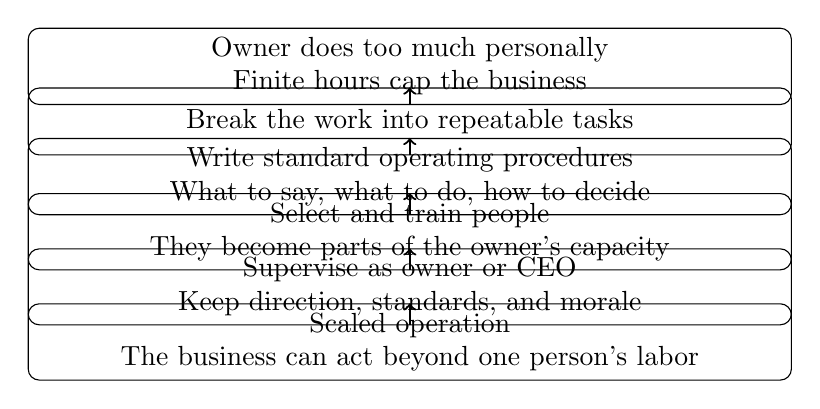
\begin{tikzpicture}[
node distance=0.7cm,
box/.style={draw, rounded corners, align=center, text width=0.78\linewidth, minimum height=0.85cm},
arrow/.style={->, thick}
]
\node[box] (limit) {Owner does too much personally\\Finite hours cap the business};
\node[box, below of=limit] (tasks) {Break the work into repeatable tasks};
\node[box, below of=tasks] (sop) {Write standard operating procedures\\What to say, what to do, how to decide};
\node[box, below of=sop] (people) {Select and train people\\They become parts of the owner's capacity};
\node[box, below of=people] (supervise) {Supervise as owner or CEO\\Keep direction, standards, and morale};
\node[box, below of=supervise] (scale) {Scaled operation\\The business can act beyond one person's labor};
\draw[arrow] (limit) -- (tasks);
\draw[arrow] (tasks) -- (sop);
\draw[arrow] (sop) -- (people);
\draw[arrow] (people) -- (supervise);
\draw[arrow] (supervise) -- (scale);
\end{tikzpicture}
\caption{Transcript-grounded reconstruction of AK's scaling mechanism: finite owner time must be converted into repeatable procedures, trained people, and continuing leadership.}
\end{figure}

\subsection{Question \& Answer}

\paragraph{Question.}
Is a standard operating procedure enough to scale?

\paragraph{Answer.}
No. AK names SOPs as a requirement, but he immediately adds the limitation. No one will run the company exactly the way the founder runs it. Even with procedures, a change in leadership can send a company down. The owner or CEO still has to supervise direction, inspire managers, and make sure people have the right information and tools.

Thus the mechanism is:
\begin{equation}
\mathrm{Scale}
=
f(\mathrm{SOPs},\mathrm{selection},\mathrm{training},\mathrm{supervision}).
\end{equation}
The lecture's practical warning is that leaving out the final term changes the result. Procedures without leadership are brittle.

\section{Risk, The First Business, And The First Million}

The interview then turns to mentorship and money. AK's father told him, when he was entering medical school, that if he did it only for himself, falling down might become comfortable. But if he carried the flag of family, community, country, or world, then falling down would not be the end. He would look up, see what he was carrying, and get back up.

This fatherly rule becomes the motivational side of risk. When asked about the most money he made in a single year, AK resists precision. He says there are good years and bad years, that people may hear ``a couple million'' and misunderstand, and that taxes and reinvestment matter. The safe transcript-backed notation is:
\begin{equation}
I_{\mathrm{best\ year}} \approx \hbox{``a couple million''},
\end{equation}
with the immediate qualification:
\begin{equation}
\mathrm{Spendable\ income} \neq \mathrm{gross\ income}.
\end{equation}
Taxes and reinvestment reduce what can be treated as available personal spending.

When asked for the best financial decision he ever made, AK answers: the first one, the first business. He invokes the saying that the first million is the hardest, because once one has money, one has comfort and can invest in other projects. But the transcript does not reduce this to luck. It gives a risk discipline.

\subsection{A Worked Risk Rule}

Let \(K\) be capital available for a first serious business move. Let \(L\) be the possible loss, \(B\) the backup plan, and \(R\) the reinvestment needed for growth. A cautious reconstruction of AK's rule is not ``maximize the bet,'' but:
\begin{align}
&\hbox{save capital},\\
&\hbox{estimate downside } L,\\
&\hbox{prepare to lose } L,\\
&\hbox{keep backup plan } B,\\
&\hbox{remove ego from the decision},\\
&\hbox{reinvest enough } R \hbox{ that the business can grow.}
\end{align}

The update rule after a failed or difficult attempt is:
\begin{equation}
\mathrm{Skill}_{t+1}
=
\mathrm{Skill}_{t}
+
\Delta(\mathrm{attempt},\mathrm{loss},\mathrm{correction}).
\end{equation}
This is a standard reconstruction of AK's spoken claim: sometimes one loses, sometimes one wins, but without trying one does not learn the skill set needed to keep growing.

\section{Accountability As Self-Improvement}

The next question asks for the secret to self-improvement. AK again returns to his father. The rule is: never point fingers. There is always blame to go around, but the useful question is what one could have done differently.

This is a learning algorithm. If a project fails and the only output is blame, the operator does not improve. If the same failure is converted into a better selection rule, a better training rule, more background work, or harder execution, then failure has been transformed into information.

We can write the rule as:
\begin{equation}
\mathrm{Growth}
\propto
\mathrm{Accountability}
\times
\mathrm{Correction}.
\end{equation}
If accountability is zero, correction rarely begins. This is why AK says that if one always thinks everybody else did everything wrong, one never gets better.

\section{Stages Of The Entrepreneurial Problem}

AK's answer about entrepreneurial challenge is staged. The early challenge is getting started: knowledge, money, and the character not to squander what is handed over. He gives a hypothetical example:
\begin{equation}
C_{\mathrm{starter\ example}}=\$1{,}000{,}000.
\end{equation}
Even if someone receives a million dollars and the books or teaching needed to begin, AK says many will still fail because they become greedy, emotional, unreliable, idle, or unable to meet deadlines.

The next challenge is diversification. The stakes grow. A first move may require tens or hundreds of thousands. Later, one may be betting around a million dollars and risking what earlier work created. Then the challenge becomes risk calculation.

The final challenge is balance after success. AK states the thought experiment:
\begin{equation}
W_{\mathrm{retirement}}=\$10{,}000{,}000.
\end{equation}
At that point a person might be able to retire, but may not be built to stop. The real question becomes how to put life together: relationships, children, parents, and time.

\begin{table}
\centering
\begin{tabular}{|p{0.25\linewidth}|p{0.31\linewidth}|p{0.31\linewidth}|}
\hline
Stage & Main Question & Failure Mode \\
\hline
Starting & How do I get knowledge and money? & Never beginning, or lacking a plan \\
\hline
Character & Can I be trusted with opportunity? & Greed, emotion, missed deadlines, idleness \\
\hline
Diversifying & Should I bet bigger now or later? & Mispriced risk and financial ruin \\
\hline
Post-success & What is life for after enough money? & Losing family, health, or balance \\
\hline
\end{tabular}
\caption{AK's staged account of entrepreneurial difficulty. The problem changes as capital, competence, and optionality increase.}
\end{table}

\section{Reputation, History, And What Money Is For}

The last part of the interview broadens the lens. Asked whom he would spend a day with, AK names Benjamin Franklin. The point of the answer is reputation and diplomacy. AK admires Franklin as an inventor, statesman, and diplomat, and he frames him as someone respected enough that different powers would come back to the table when he spoke. This should be preserved as AK's admiration and claim, not expanded into independent historical proof.

The mechanism AK extracts is simple: make something of yourself, be honest, treat people fairly, and become the kind of person whose words are worth hearing. In the language of the chapter:
\begin{equation}
\mathrm{Influence}
\approx
g(\mathrm{competence},\mathrm{honesty},\mathrm{fairness},\mathrm{trust}).
\end{equation}

The world-history answer continues the same theme. AK says humans keep being fooled by the same tricks: people seeking power divide others, sell narratives, provoke emotional decisions, and make people fight over hard ideological lines. The practical lesson is not cynicism. It is constructive judgment: understand why the other side sees what it sees, then ask what can be done to make things better.

The final question returns to his father. The greatest lesson is not to get caught up with the money. AK offers a final identity experiment:
\begin{equation}
W_{\mathrm{identity}}=\$100{,}000{,}000.
\end{equation}
Suppose that money is taken away. What remains? The answer he wants to preserve is not the account balance, but the person: whether others still say that he helped, looked out for people, was a good friend, and was a good family member.

\section{Summary}

The interview begins with cars, but it does not end there. Its real arc is a theory of conversion: direct professional labor becomes durable institutions through operations; owner capacity becomes organizational capacity through SOPs, selection, training, and supervision; risk becomes skill when it is calculated and survived; failure becomes growth when it is met with accountability; and money becomes dangerous if it replaces health, family, reputation, and character.

For the larger book, AK's contribution is strongest on five durable questions: what a person actually controls, how scale is built, how risk is financed and survived, which operating discipline compounds fastest, and what wealth is for after the number is reached. The answer, in his telling, is that money should remain a byproduct of useful work and personal growth. The protected asset is the person who remains after the money arrives.